\documentclass[fr]{../../../../../../eplexam}

\hypertitle{Théorie et algorithmique des graphes}{5}{INMA}{1691}{2018}{Janvier}{Mineure}
{Gilles Peiffer, Romain Graux}
{Vincent Blondel et Jean-Charles Delvenne}

Veuillez expliquer vos raisonnements avec clarté,
répondre à des questions différentes sur des feuilles \emph{différentes},
sans oublier d'apposer \emph{votre nom} sur chacune.

\section{Question 1}
Deux alpinistes Henri et Brieuc sont de part et d'autre
d'une chaîne de montagnes,
à l'altitude zéro, et souhaitent échanger leurs positions,
avec la fantaisie suivante: à tout moment
ils souhaitent être l'un et l'autre à la même altitude.
On modélise la chaîne de montagnes dans le plan discret
comme une suite d'\og escaliers \fg{} montants ou descendants.
Chaque marche a une coordonnée horizontale $x \in 0, 1, \ldots, N-1$
et une altitude $z \in \{\,0, 1, 2, \ldots\,\}$
(l'altitude ne descend donc jamais en dessous de zéro).
Deux marches successives ont toujours
une différence d'altitude de $1$ exactement.

À chaque temps $t = 0, 1, 2, \ldots$,
chaque alpiniste avance ou recule de $1$,
et donc monte ou descend de $1$:
$\abs{x_{\textnormal{Henri}}(t+1) - x_{\textnormal{Henri}}(t)} = 1$
et $\abs{z_{\textnormal{Henri}}(t+1) - z_{\textnormal{Henri}}(t)} = 1$,
et de même pour Brieuc.
Ils sont initialement en $x=0$ et $x=N-1$ respectivement.

Considérez le graphe dont les n\oe{}uds sont les couples (paires ordonnées)
de marches à la même altitude.
Deux n\oe{}uds $(u_1, u_2)$ et $(v_1, v_2)$ sont reliés
s'il est possible pour Henri et Brieuc
sur les marches $u_1$ et $u_2$ respectivement
de passer en une étape aux marches $v_1$ et $v_2$.

\begin{enumerate}
	\item Démontrez que chaque n\oe{}ud de ce graphe
	a un degré de $0$, $1$, $2$ ou $4$,
	et qu'il y a exactement quatre n\oe{}uds de degré $1$.
	Quels sont ces n\oe{}uds?
	\item Démontrez que dans tout graphe
	avec exactement deux n\oe{}uds de degré impair,
	ces deux n\oe{}uds font partie de la même composante connexe.
	\item Démontrez que Henri et Brieuc
	peuvent bien échanger leurs positions
	en restant à tout moment à la même hauteur l'un que l'autre.
\end{enumerate}

\nosolution

\section{Question 2}

Le Choixpeau magique est chargé, au collège de Poudlard, de répartir les 50 nouveaux étudiants entre les quatre maisons Serpentard, Serdaigle, Poufsouffle et Gryffondor. La chose n’est pas simple car certaines paires d’élèves, par exemple Potter et Malefoy, éprouveraient une certaine répulsion à l’idée de devoir cohabiter.

Albus Dumbledore, le directeur de l’établissement, trace d’un air songeur un graphe des étudiants en conflit, en reliant par exemple les noms de Potter et Malefoy. Il remarque que ce graphe de 50 noeuds est connexe et 4-régulier (chaque étudiant est en conflit avec exactement 4 autres étudiants).

\begin{enumerate}
	\item Montrez que le Choixpeau magique peut proposer une répartition qui évite tout conflit dans une maison.
	\item Severus Rogue, l’austère professeur de Potions, se dit qu’il serait plus formateur d’introduire une saine émulation au sein de certaines maisons qu’inondent un peu trop l’entraide et la joie de vivre. Il propose de trouver un élève dans le graphe, de façon à ce que les autres étudiants
	se retrouvent répartis en exactement trois composantes connexes. L’élève irait alors seul à Serpentard ; l’une des composantes connexes serait attribuée à la maison Gryffondor, l’autre à Poufsouffle, la troisième à Serdaigle. Démontrez que le plan du Prof. Rogue n’est pas possible. Le théorème des poignées de main pourrait vous être utile.
\end{enumerate}

\nosolution

\section{Question 3}

La Commission Européenne doit de toute urgence traduire un communiqué de presse du français dans huit autres langues européennes : l’anglais, l’espagnol, l’italien, le finnois, le suédois, le portugais, le hongrois et le letton.
Les traducteurs Alphonse, Bertrand, Charline, Donald, Emilie, Fleur, Gérard et Henriette sont diponibles. La liste des langues maîtrisées par les traducteurs sont indiquées sur la figure ci-dessous. Chaque traducteur, en une journée de travail, peut traduire vers une autre langue.
Comment assigner les langues aux traducteurs de façon à disposer d’un maximum de traductions après un jour? Combien de jours faudra-t-il au minimum pour tout traduire? Démontrez vos affirmations.

\begin{figure}[H]
	\centering
	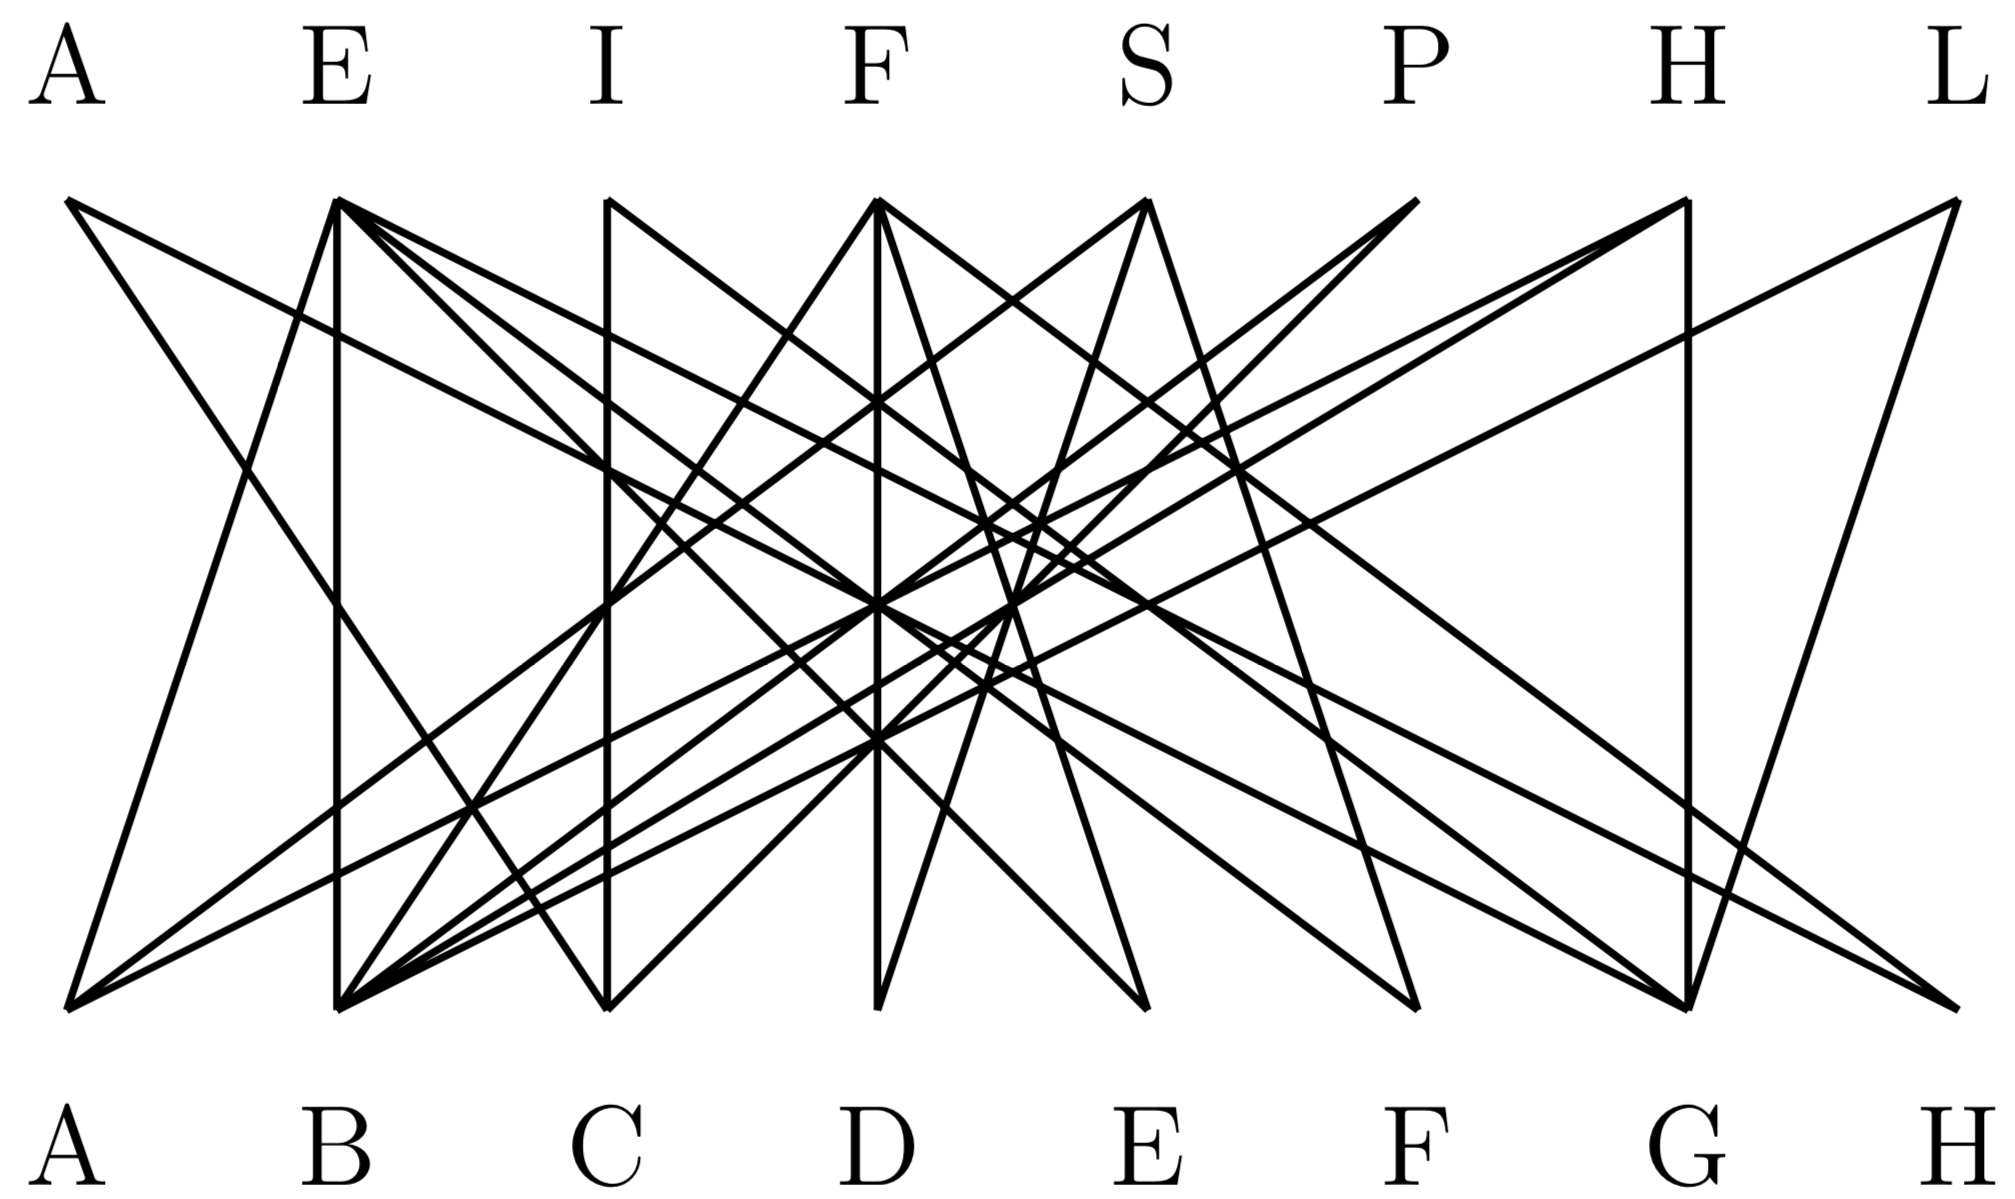
\includegraphics[width=0.5\textwidth]{./imgs/graphe.png}
\end{figure}

\begin{solution}
	Une solution peut être la suivante:
	\begin{figure}[H]
		\centering
		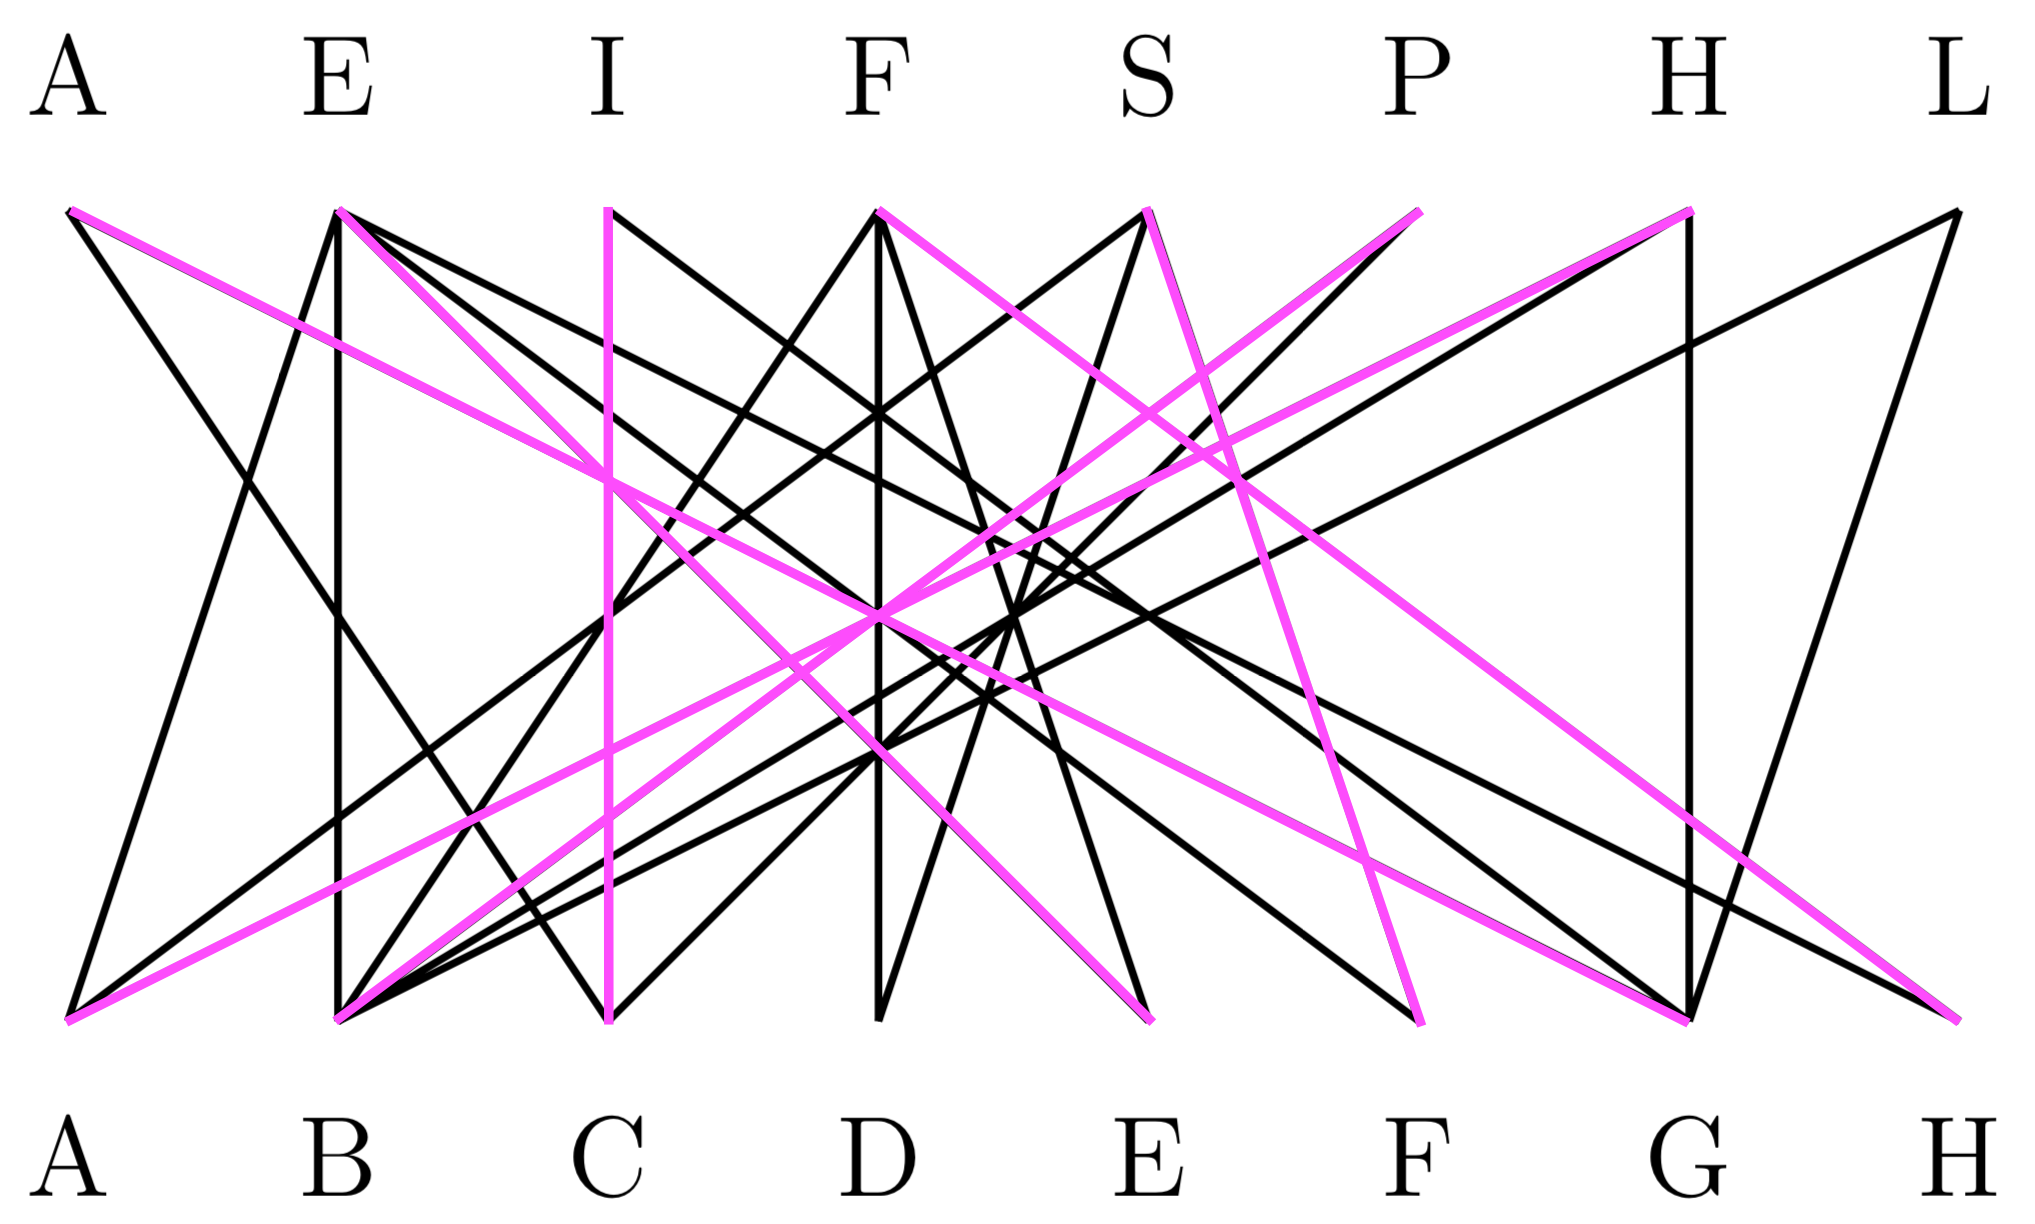
\includegraphics[width=0.5\textwidth]{./imgs/grapheSol.png}
	\end{figure}

	Pour déterminer si ce couplage est maximal, prenons le sous graphe suivant avec toutes ses arêtes adjacentes:
	\begin{figure}[H]
		\centering
		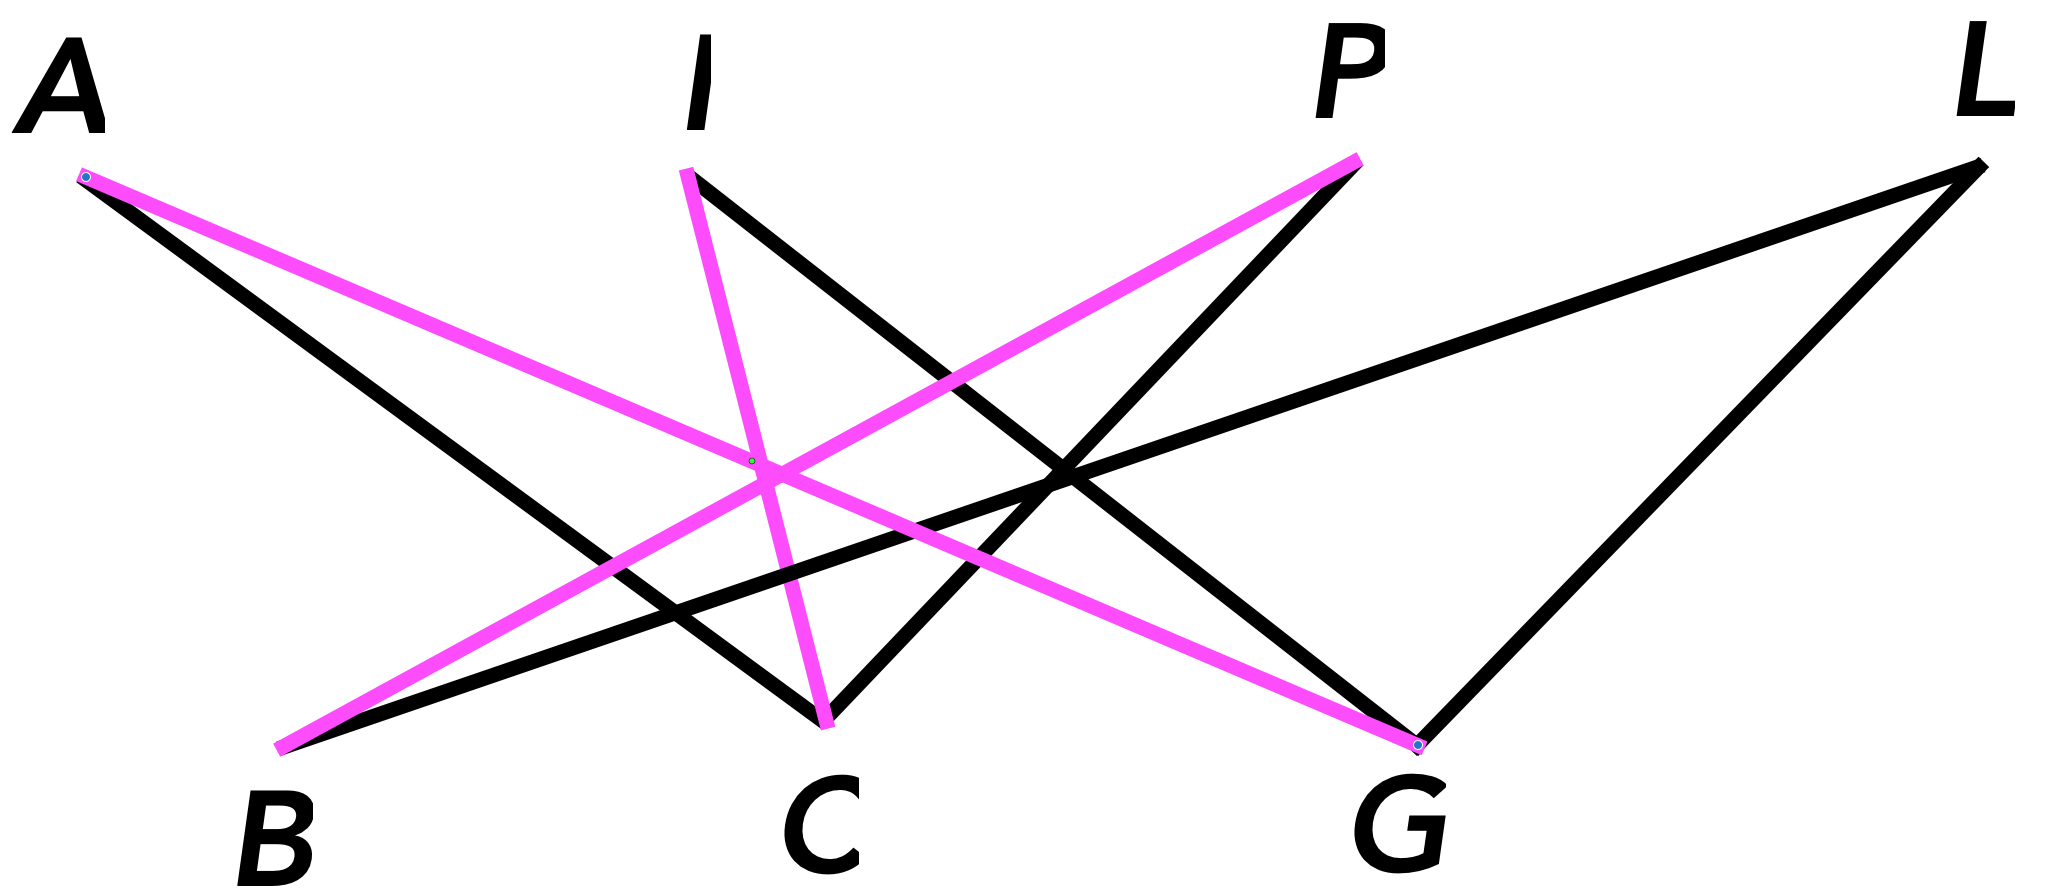
\includegraphics[width=0.5\textwidth]{imgs/sousGraphe.png}
	\end{figure}
	De ce sous-graphe on peut bien se rendre compte qu'il n'y a pas de couplage M-augmenté, le couplage est donc maximum mais pas parfait, les traductions se feront donc sur 2 jours.
\end{solution}


\section{Question 4}

Vrai ou faux? Justifiez.

\begin{enumerate}
	\item Sentant sa mort venir Nabuchodonosor IV, roi de Babylone, partitionna son pays, vaste territoire d’un seul tenant, en 5 royaumes d’un seul tenant pour ses 5 fils, de sorte que chaque prince avait une frontière commune (non réduite à un point) avec chacun des territoires des ses frères.
	\item Il existe un graphe simple à 6 noeuds dont les degrés sont 1, 2, 3, 4, 4, 5.
	\item Si P $\neq$ NP, alors vérifier qu’un graphe donné possède une clique de 100 noeuds est aussi difficile (en terme de temps de calcul asymptotique requis, et à une transformation polyno- miale près) que celui de vérifier qu’un graphe donné est hamiltonien.
	\item Le graphe de l’hypercube de dimension n $\geq$ 1 (dont les noeuds sont les points de coordonnées binaires de $R^n$ et les arêtes relient les noeuds à distance euclidienne unité) est hamiltonien pour tout n.
	\item Un arbre de degré maximum 10 possède toujours un coloriage propre d’arêtes à 10 couleurs.
	\item Bonus : un graphe complet à n $\geq$ 3 noeuds dont chaque arête est coloriée en bleu ou rouge possède toujours un cycle hamiltonien qui est monochrome ou qui est l’union de deux chemins monochromes.
\end{enumerate}

\begin{solution}
	\begin{enumerate}
		\item Faux : On peut représenter cet agencement en tant que graphe, les noeuds représentant le territoire d'un frère et les arêtes étant les frontières entre eux. Pour que chaque frère ai une arête avec chacun de ses frères, ce graphe est un graphe complet $K_5$, ce graphe n'étant pas planaire, il est impossible pour ces frères d'avoir une frontière en commun avec chacun de ces frères et gardant son pays en un seul tenant.
		\item Faux : $\sum d_i = 19$ (impaire), d'après le théorème des poignées de main, impossible.
		\item Ok google
		\item Vrai
		\item Vrai : étant donné que chaque arête doit se finir quelque part, c'est une feuille.
		Procédons par récurrence.
		Initialisation: Lorsqu'il n'y a qu'un seul n\oe{}ud,
		le degré maximum vaut $1$ et il y a une feuille.
		Induction: admettons que la propriété soit vraie
		pour $\Delta(G) = n-1$.
		Si l'on rajoute un n\oe{}ud
		et qu'on trace une arête vers un n\oe{}ud
		qui n'est pas de degré maximal,
		le graphe possèdera une feuille en plus.
		Si l'on rajoute un n\oe{}ud
		et qu'on trace une arête vers un n\oe{}ud est de degré maximal,
		le graphe possèdera une feuille en plus
		et le degré maximal aura augmenté d'un aussi.
		Nous avons donc
		dans tous les cas $n_{\textnormal{feuilles}} \ge \Delta(G)$.
		\item
	\end{enumerate}
\end{solution}

\end{document}
